\documentclass[handout,compress]{beamer}

\usetheme[block=fill]{metropolis}

\usepackage{graphicx} % Allows including images
\usepackage{amsmath,amsfonts,amsthm,amssymb}
\usepackage{color}
\usepackage{xcolor,cancel}
%\setitemize{label=\usebeamerfont*{itemize item}%
%	\usebeamercolor[fg]{itemize item}
%	\usebeamertemplate{itemize item}}
\definecolor{mDarkBrown}{HTML}{604c38}
\definecolor{mDarkTeal}{HTML}{23373b}
\definecolor{mLightBrown}{HTML}{EB811B}
\definecolor{mMediumBrown}{HTML}{C87A2F}
\definecolor{mygreen}{HTML}{98C2B9}
\definecolor{myyellow}{HTML}{DFD79C}
\definecolor{myblue}{HTML}{8CA7CC}
\definecolor{kern}{HTML}{8CC2B7}

\usepackage{float}
\usepackage{framed}
\usepackage{epsfig}
\usepackage{graphicx}
\usepackage{subcaption}
\usepackage{ulem}
\usepackage{hhline}
\usepackage{multirow}
\usepackage{comment}   
\usepackage{bbm}
\usepackage{tikz}   
\usepackage{ulem}
\def\Put(#1,#2)#3{\leavevmode\makebox(0,0){\put(#1,#2){#3}}}
\newcommand*\mystrut[1]{\vrule width0pt height0pt depth#1\relax}
\newcommand{\eqdef}{\mathbin{\stackrel{\rm def}{=}}}


\newcommand{\bs}[1]{\boldsymbol{#1}}
\newcommand{\bv}[1]{\mathbf{#1}}
\newcommand{\R}{\mathbb{R}}
\newcommand{\E}{\mathbb{E}}

\DeclareMathOperator*{\argmin}{arg\,min}
\DeclareMathOperator*{\argmax}{arg\,max}
\DeclareMathOperator{\nnz}{nnz}
\DeclareMathOperator{\Var}{Var}
\DeclareMathOperator{\sinc}{sinc}
\DeclareMathOperator{\mv}{mv}
\DeclareMathOperator{\sgn}{sgn}
\DeclareMathOperator{\step}{step}
\DeclareMathOperator{\gap}{gap}
\DeclareMathOperator{\poly}{poly}
\DeclareMathOperator{\tr}{tr}
\DeclareMathOperator{\orth}{orth}
\newcommand{\norm}[1]{\|#1\|}
\captionsetup[subfigure]{labelformat=empty}
\captionsetup[figure]{labelformat=empty}
\DeclareMathOperator*{\lmin}{\lambda_{min}}
\DeclareMathOperator*{\lmax}{\lambda_{max}}

\newcommand{\specialcell}[2][c]{%
  \begin{tabular}[#1]{@{}c@{}}#2\end{tabular}}
\newcommand{\specialcellleft}[2][c]{%
\begin{tabular}[#1]{@{}l@{}}#2\end{tabular}
}

\usepackage{tabstackengine}
\stackMath


%----------------------------------------------------------------------------------------
%	TITLE PAGE
%----------------------------------------------------------------------------------------

\title{CS-UY 4563: Lecture 6 \\ Naive Bayes, the Bayesian Perspective}
\author{NYU Tandon School of Engineering, Prof. Christopher Musco}
\date{}

\begin{document}

\begin{frame}
	\titlepage 
\end{frame}

\metroset{titleformat=smallcaps}

\begin{comment}
\end{comment}

\begin{frame}[t]
	\frametitle{model selection lab}
	Lab 3, due \textbf{Next Thursday}.
	\begin{center}
		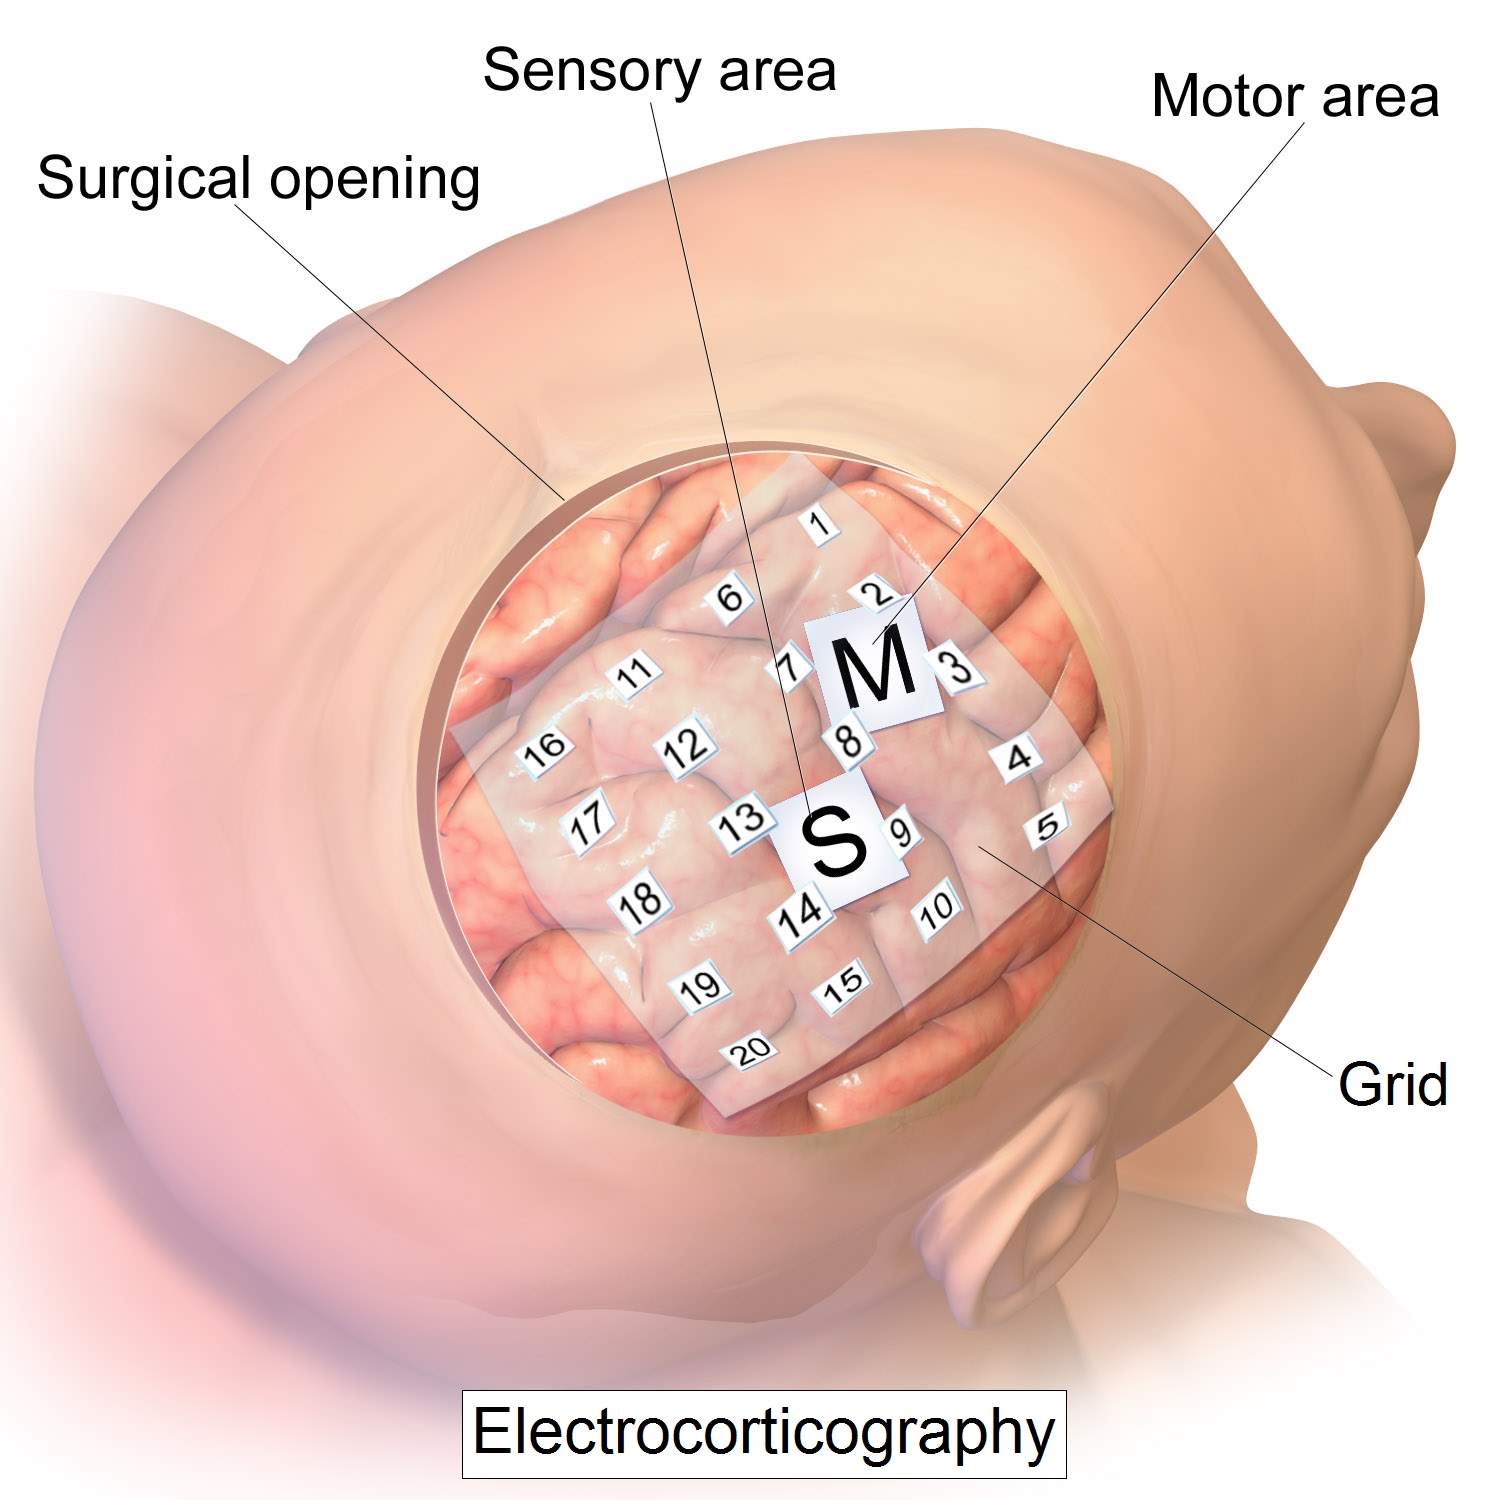
\includegraphics[width=.3\textwidth]{eocg.png}
	\end{center}
	\begin{itemize}
		\item Predict hand motion based on electrical measurements of a monkeys brain activity.
		\item Experience working with sequential (time series) data.
		\item First lab where computation actually matters (solving regression problems with ~ 40k examples, 1500 features)
	\end{itemize} 
\end{frame}

\begin{frame}
	\frametitle{over-parameterized models}
	\begin{center}
		If you have enough features, even \emph{most basic model} will overfit in practice.
		
		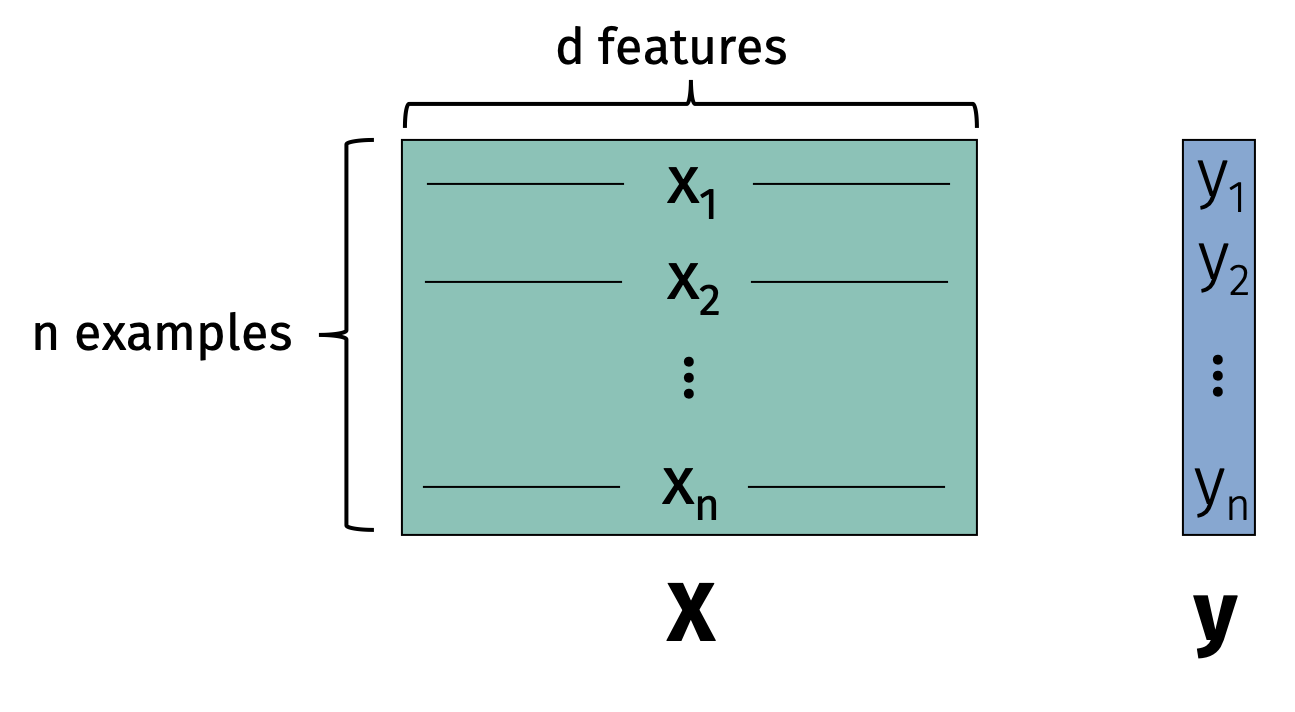
\includegraphics[width=.5\textwidth]{overparameterized.png}
		
		\textbf{Example:} Linear regression model where $d \geq n$. Can always find $\bs{\beta}$ so that $\bv{X}\bs{\beta} = \bv{y}$ exactly. 
	\end{center}
\end{frame}

\begin{frame}
	\frametitle{avoiding overfitting}
	\textbf{Regularization:}
	Explicitly discourage overfitting by adding a \emph{regularization penalty} to the loss minimization problem.  
	\begin{align*}
		\min_{\bs{\theta}} \left[ L(\bs{\theta}) \alert{+ Reg(\bs{\theta})} \right].
	\end{align*}
	
	\textbf{Example:} Least squares regression. $L(\bs{\beta}) = \|\bv{X}\bs{\beta} - \bv{y}\|_2^2$.
	\begin{itemize}
		\item Ridge regression ($\ell_2$): \alert{$Reg(\bs{\beta}) = \lambda \|\bs{\beta}\|_2^2$}
		\item LASSO ($\ell_1$): \alert{$Reg(\bs{\beta}) = \lambda \|\bs{\beta}\|_1$}
		\item Elastic net: \alert{$Reg(\bs{\beta}) = \lambda_1 \|\bs{\beta}\|_1 + \lambda_2 \|\bs{\beta}\|_2^2$}
	\end{itemize}
\end{frame}

\begin{frame}
	\frametitle{ridge regularization}
	\begin{center}
		Ridge regression: $\min_{\bs{\beta}} \|\bv{X}\bs{\beta} - \bv{y}\|_2^2 + \lambda \|\bs{\beta}\|_2^2$.
	\end{center}
\begin{itemize}
	\item Minimized at $\bs{\beta} = (\bv{X}^T\bv{X} + \lambda\bv{I})^{-1}\bv{X}^T\bv{y}$. 
	\item Let $\bs{\beta}^* = \argmin_{\bs{\beta}} L(\bs{\beta})$ and $\alert{\bs{\beta}_R^* = \argmin_{\bs{\beta}} L(\bs{\beta}) + Reg(\bs{\beta})}$. 
	\item Always have  $\alert{\|\bs{\beta}_R^*\|_2^2} < \|\bs{\beta}^*\|_2^2$ and $\alert{\|\bv{X}\bs{\beta}_R^* - \bv{y}\|_2^2} > \|\bv{X}\bs{\beta}^* - \bv{y}\|_2^2$.
\end{itemize}
\vspace{-1em}
	\begin{center}
	Feature selection methods attempt to set many coordinates in $\bs{\beta}$ to 0. Regularization encourages coordinates to be small. 
	\end{center}
\end{frame}

\begin{frame}
	\frametitle{lasso regularization}
		\begin{center}
		Lasso regularization: $\min_{\bs{\beta}} \|\bv{X}\bs{\beta} - \bv{y}\|_2^2 + \lambda \|\bs{\beta}\|_1$.
	\end{center}
	\begin{itemize}
		\item Similarly encourages coordinates in $\bs{\beta}$ to be small. 
		\item Often the optimal $\bs{\beta}_R^*$ will have subset of coordinates equal to zero, in contrast to ridge regularization.
	\end{itemize}
	\vspace{-1em}
	\begin{center}
		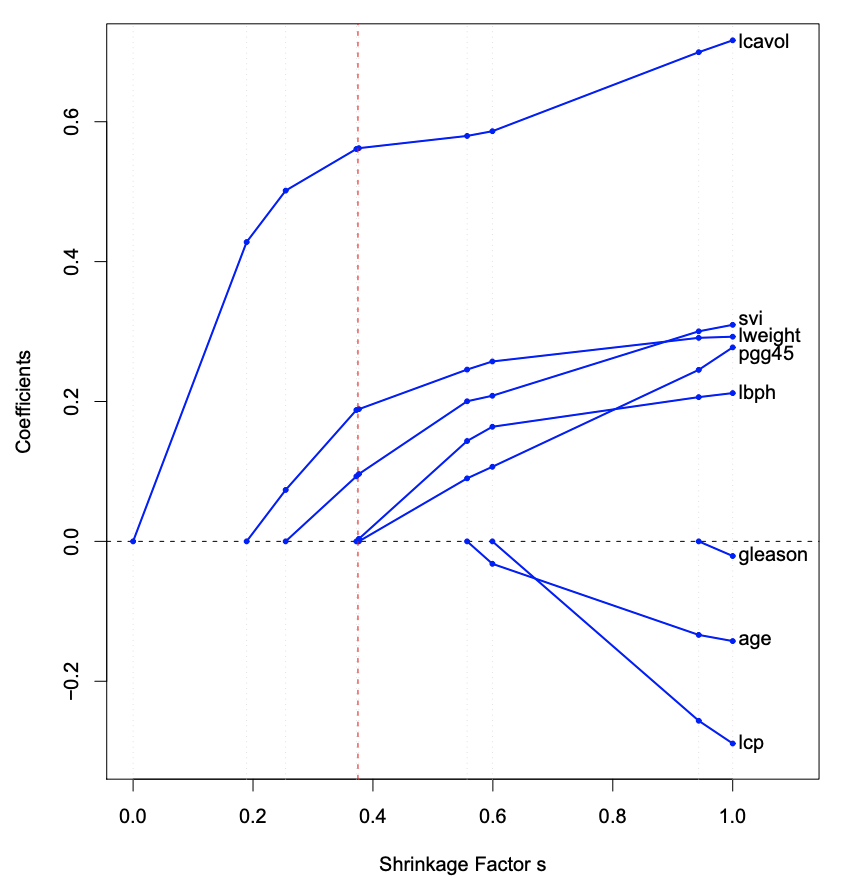
\includegraphics[width=.4\textwidth]{lasso_coeffs.png}
	\end{center}
\end{frame}

\begin{frame}
	\frametitle{lasso regularization}
	\textbf{Pros:}
	\begin{itemize}
		\item Simpler, more interpretable model.
	\end{itemize}

	\textbf{Cons:}
\begin{itemize}
	\item No closed form solution because $\|\bs{\beta}\|_1$ is not differentiable. 
	\item Can be solved with iterative methods (gradient descent), but generally not as quickly as ridge regression.
\end{itemize}
	
\end{frame}

\begin{frame}[standout]
	\begin{center}
		\large classification
	\end{center}
\end{frame}

\begin{frame}
	\frametitle{classification setup}
	\begin{itemize}
		\item \textbf{Data Examples:} $\bv{x}_1,\ldots, \bv{x}_n \in\R^d$
		\item \textbf{Target:} $y_1, \ldots, y_n \in \{0,2,\ldots, q-1\}$ when there are $q$ classes.
		\begin{itemize}
			\item Binary Classification: $q = 2$, so each $y_i \in \{0,1\}$.
			\item Multi-class Classification: $q > 2$. \footnote{Note that there is also \emph{multi-label} classification where each data example maybe belong to more than one class.}
		\end{itemize}
	\end{itemize}
\end{frame}

\begin{frame}
	\frametitle{classification examples}
	\begin{itemize}
		\item Medical diagnosis from MRI: 2 classes.
		\item MNIST digits: 10 classes.
		\item Full Optical Character Regonition: 100s of classes.
		\item ImageNet challenge: 21,000 classes.
	\end{itemize}
\begin{center}
	\textbf{Running example today: \alert{Email Spam Classification.}}
\end{center}
\end{frame}

\begin{frame}
	\frametitle{classification}
	\begin{center}
		\textbf{Today:} ML from a \textbf{\alert{Probabilistic/Bayesian Perspective}}.
	\end{center} 
	
	\begin{center}
	Classification can (and often is) solved using the same \textbf{loss-minimization framework} we saw for regression. 
	\end{center}

	We won't see that today! We're going to use classification as a window into another way of thinking about machine learning.
\end{frame}

\begin{frame}
	\frametitle{spam prediction}
	\begin{center}
		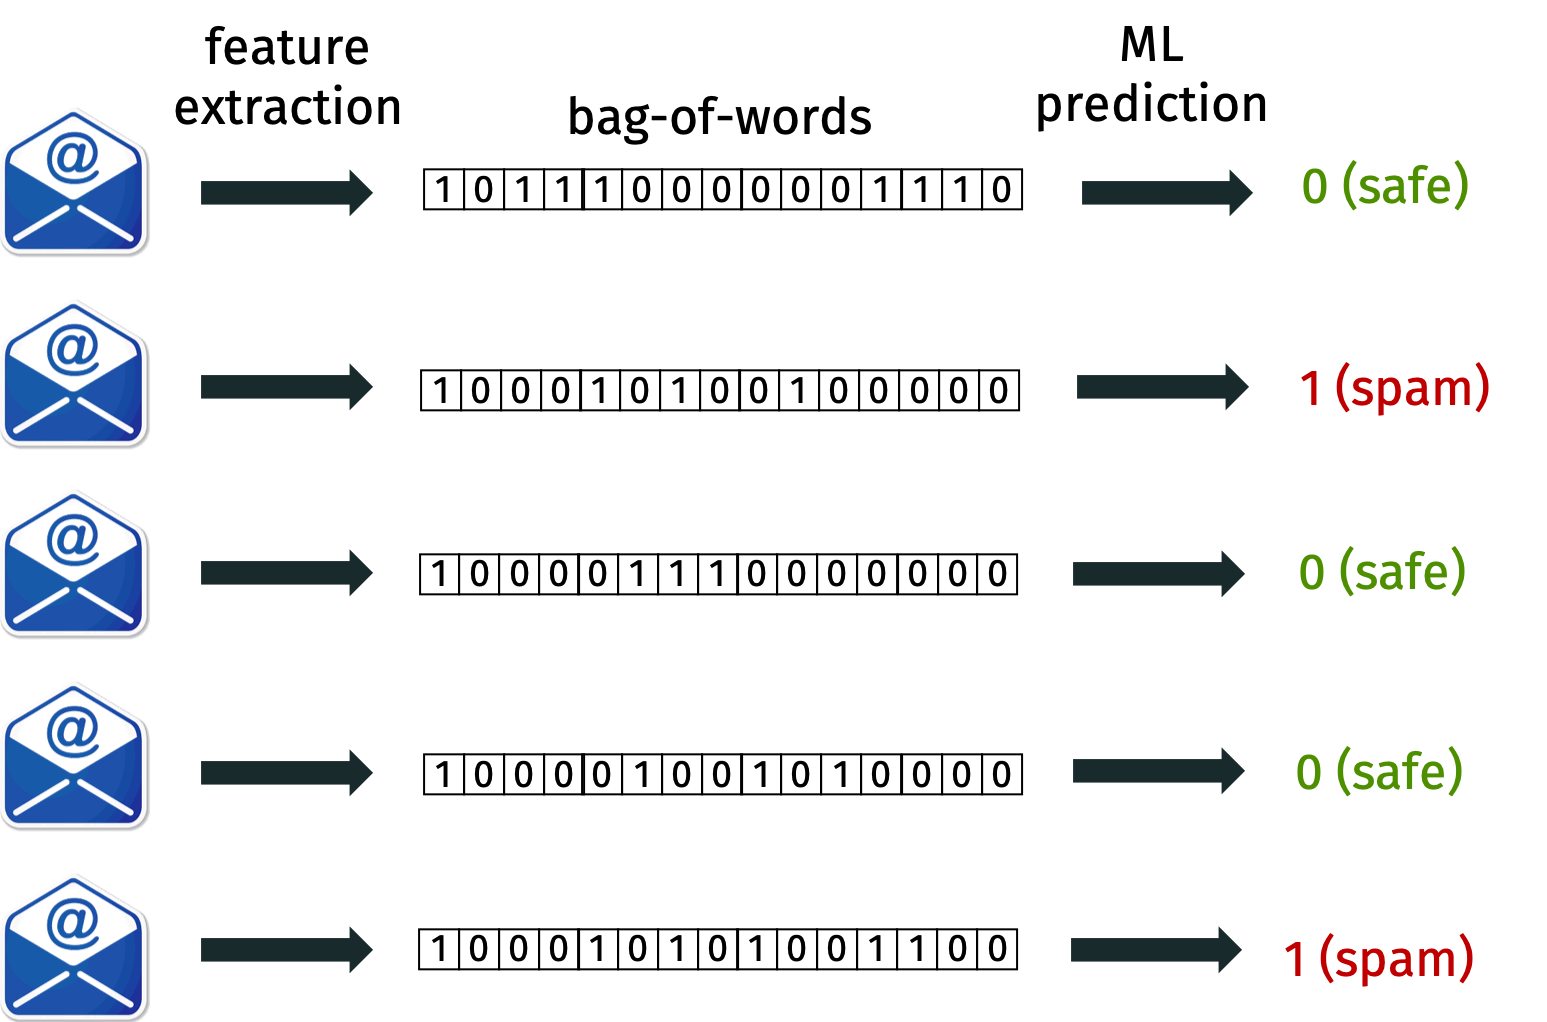
\includegraphics[width=.9\textwidth]{spam.png}
		
		\vspace{.5em}
		\textbf{Both target labels \emph{and} data vectors are binary.}
	\end{center}
\end{frame}

\begin{frame}
	\frametitle{spam prediction}
	\textbf{First Goal:} Model data $(\bv{x},y)$ -- in our case emails -- as a \emph{simple} probabilistic process. \alert{\textbf{Probabilistic Modeling.}}
	
	\begin{center}
		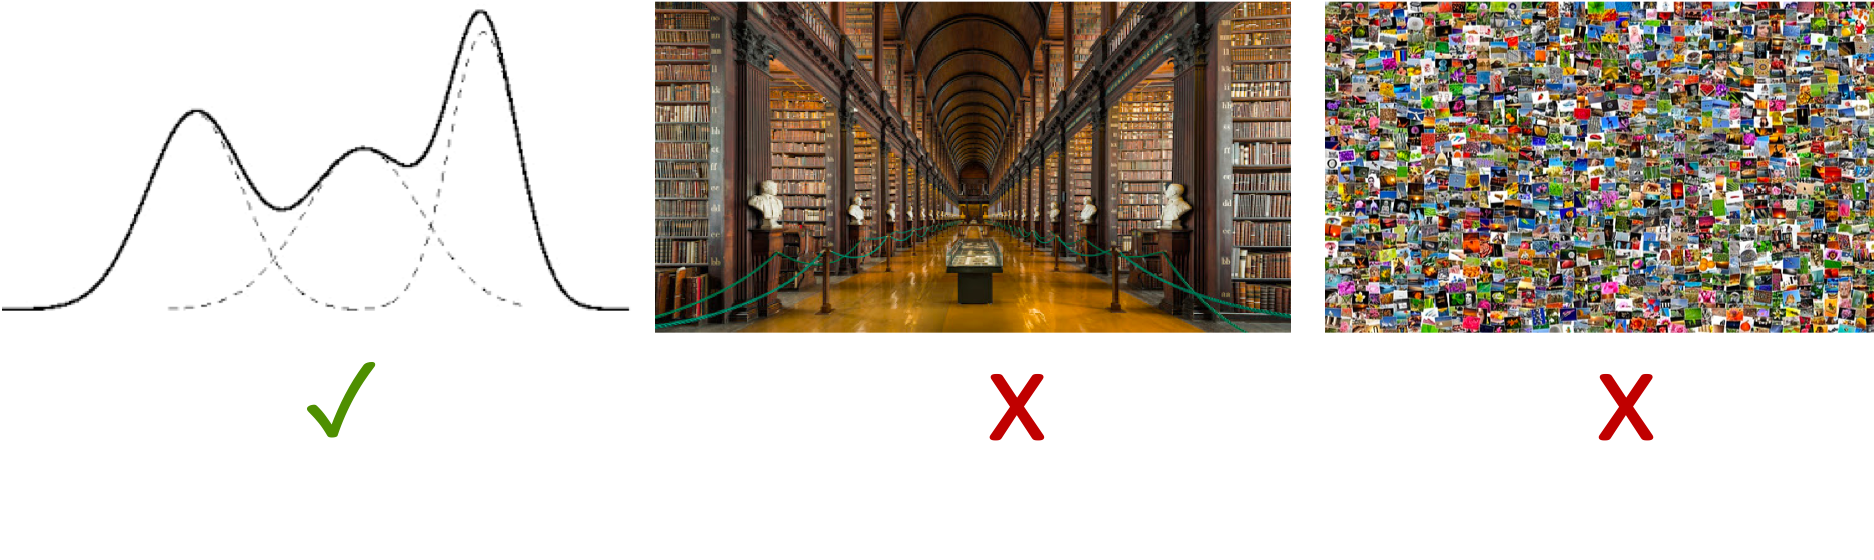
\includegraphics[width=.9\textwidth]{data_dists.png}
		
		How would you randomly create a set of email feature vectors and labels (from scratch) that looks like a typical inbox? 
		
		Should have some spam emails, and some regular emails. 
	\end{center}
\end{frame}

\begin{frame}
	\frametitle{probabilistic model for email}
	Random model for generating data example $(\bv{x},y)$:
	\begin{itemize}
		\item Set $y = 0$ with probability $p_0$, $y = 1$ with probability $p_1 = 1-p_0$. 
		\begin{itemize}
			\item $p_0$ is probability an email is not spam (e.g. $99\%$). 
			\item $p_1$ is probability an email is spam (e.g. $1\%$). 
		\end{itemize}
		\item If $y=0$, for each $i$, set $x_i = 1$ with probability $p_i^{(0)}$.
		\item If $y=1$, for each $i$, set $x_i = 1$ with probability $p_i^{(1)}$.
	\end{itemize}
	Each index $i$ corresponds to a different word. For what words would we expect $p_i^{(1)} > p_i^{(0)}$? $p_i^{(0)} > p_i^{(1)}$?
\end{frame}

\begin{frame}
	\frametitle{probability review}
	\begin{itemize}
		\item \textbf{Probability:} p(x) -- the probability event $x$ happens.
		\item \textbf{Joint probability:} p(x,y) -- the probability that event $x$ \emph{and} event $y$ happen. 
		\item \textbf{Conditional Probability} $p(x \mid y)$ -- the probability $x$ happens \emph{given} that $y$ happens.
	\end{itemize}

\begin{align*}
	p(x | y) = 
\end{align*}

\end{frame}

\begin{frame}
	\frametitle{bayes theorem/rule}
	\begin{itemize}
		\item $p(x | y) = \frac{p(x,y)}{p(y)}$
		\item $p(y | x) = \frac{p(x,y)}{p(x)}$
	\end{itemize}
\textbf{So:}
\begin{align*}
	p(x | y) = \frac{p(y | x)p(x)}{p(y)}
\end{align*}
\end{frame}

\begin{frame}
	\frametitle{probabilistic model for email}
	Random model for generating data example $(\bv{x},y)$:
	\begin{itemize}
		\item Set $y = 0$ with probability $p(C_0)$, $y = 1$ with probability $p(C_1) = 1-p(C_0)$. 
		\begin{itemize}
			\item $p(C_0)$ is probability an email is not spam (e.g. $99\%$). 
			\item $p(C_1)$ is probability an email is spam (e.g. $1\%$). 
		\end{itemize}
		\item If $y=0$, for each $i$, set $x_i = 1$ with probability $p(x_i = 1 \mid C_0)$.
		\item If $y=1$, for each $i$, set $x_i = 1$ with probability $p(x_i = 1\mid C_1)$.
	\end{itemize}
\end{frame}

\begin{frame}
	\frametitle{bayesian view on classification}
	Given unlabeled input $(\bv{x},\rule{.6cm}{0.15mm})$,choose the label $y$ which is \emph{most likely} given the data. Recall $\bv{x} = [0,0,1,\ldots, 1, 0]$. 
	
	\begin{center}
		\textbf{maximum a posterior probability (MAP) estimate}
		
		\vspace{1em}
		\alert{\textbf{Bayesian Classification Algorithm:} }
		\vspace{-.5em}
	\end{center}
	\textbf{Compute:}
	\begin{itemize}
		\item $p(C_0 | \bv{x})$: probability $y = 0$ given observed data vector $\bv{x}$. 
		\item $p(C_1 | \bv{x})$: probability $y = 1$ given observed data vector $\bv{x}$. 
	\end{itemize}
	\textbf{Output:} $C_0$ or $C_1$ depending on which probability is larger.
	
	\begin{center}
		$p(C_0 | \bv{x})$ and $p(C_1 | \bv{x})$ are called \textbf{\alert{posterior}} probabilities.
	\end{center}
\end{frame}

\begin{frame}
	\frametitle{evaluating the posterior}
	How to compute the posterior? Bayes rule!
	\begin{align}
		p(C_0 | \bv{x}) = \frac{p(\bv{x}\mid C_0)p(C_0)}{p(\bv{x})}
	\end{align}
	\begin{align}
	\text{posterior} = \frac{\text{likelihood}\times \text{prior}}{\text{evidence}}
	\end{align}
	\begin{itemize}
		\item \textbf{Prior:} Probability in class $C_0$ \emph{prior} to seeing any data.
		\item \textbf{Posterior:} Probability in class $C_0$ \emph{after} seeing the data.
	\end{itemize}
\end{frame}

\begin{frame}
	\frametitle{evaluating the posterior}
Goal is to determine which is larger:
\begin{align*}
p(C_0 | \bv{x}) &= \frac{p(\bv{x}\mid C_0)p(C_0)}{p(\bv{x})} & &\text{vs.} & \alert{p(C_1 | \bv{x}) }&\alert{= \frac{p(\bv{x}\mid C_1)p(C_1)}{p(\bv{x})} }
\end{align*}
We can ignore evidence $p(\bv{x})$ since it is the same for both sides.

\textbf{Estimate all of the other terms from the labeled data set:}
\begin{itemize}
	\item $p(C_0)=$ fraction of emails in data which are not spam.
	\item $p(C_1)=$ fraction of emails in data which are spam.
	\item $p(\bv{x} \mid C_0)=$ ?
\end{itemize}
\end{frame}

\begin{frame}
	\frametitle{naive bayes}
	``Naive'' Bayes Classifier: Approximate $p(\bv{x} \mid C_0)$ by assuming \emph{independence}:
	\begin{align*}
	p(\bv{x} \mid C_0) = p({x}_1 \mid C_0) \cdot p({x}_2 \mid C_0) \cdot \ldots \cdot p({x}_n \mid C_0)
	\end{align*}

	\begin{itemize}
		\item $p({x}_i \mid C_0)$ is the probability you observe $x_i$ given that an email is not spam.\footnote{Recall, $x_i$ is either $0$ when $word_i$ is not present, or $1$ when $word_i$ is present.} 
	\end{itemize}

A more complicated method might take dependencies into account.
\end{frame}

\begin{frame}
	\frametitle{naive bayes}
	\begin{center}
		\textbf{Final Naive Bayes Classifier}
	\end{center}
	Using data set compute:
	\begin{itemize}
		\item $p(C_0),p(C_1)$
		\item For all $i$:
		\begin{itemize}
			\item Compute $p(0 \text{ at position $i$} \mid C_0), p(1\text{ at position $i$}  \mid C_0)$
			\item Compute $p(0 \text{ at position $i$} \mid C_1), p(1\text{ at position $i$}  \mid C_1)$
		\end{itemize}
	\end{itemize}

	For prediction:
\begin{itemize}
%	\item Compute $p(C_0 | \bv{x}) $
	\item For all $i$:
	\begin{itemize}
		\item Compute $p(\bv{x}\mid C_0) = \prod_i p(x_i \mid C_0)$
		\item Compute $p(\bv{x}\mid C_1) = \prod_i p(x_i \mid C_1)$
	\end{itemize}
	\item Return 
	\begin{align*}
			\argmax \left[ p\left(\bv{x} \mid C_0\right)p\left(C_0\right), \alert{p\left(\bv{x}\mid C_1 \right)p\left(C_1\right)} \right].
	\end{align*}
\end{itemize}
\end{frame} 

\begin{frame}
	\frametitle{bayesian regression}
	The Bayesian view offers an interesting alternative perspective on \emph{many} machine learning techniques. 
	
	\vspace{2em}
	\textbf{Example:} Linear Regression. 
	
	\textbf{Probabilistic model:}
	\begin{align*}
	 	y_i = \langle \bv{x}_i, \bs{\beta} \rangle+ \eta
	\end{align*}
	where the $\eta \sim N(0,\sigma^2)$ is \textbf{random Gaussian noise}.
	\vspace{.5em}
	\begin{columns}
		\begin{column}{.5\textwidth}
				\hspace{2em}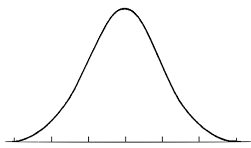
\includegraphics[width=.7\textwidth]{bell.png}
		\end{column}
		\begin{column}{.5\textwidth}
				$Pr(\eta = z) \sim$
		\end{column}
	\end{columns}
The symbol $\sim$ means ``is proportional to". 
\end{frame}

\begin{frame}
	\frametitle{bayesian regression}
		\textbf{Bayesian Goal:} Choose $\bs{\beta}$ to  maximize:
		\begin{align*}
		\Pr(\bs{\beta} \mid (\bv{X},\bv{y}) )  = \frac{\Pr((\bv{X},\bv{y}) \mid  \bs{\beta} ) \Pr(\bs{\beta} )  }{\Pr((\bv{X},\bv{y}) )}.
		\end{align*}
		
		Assume all $\bs{\beta}$'s are equally likely, so we only care about $\Pr((\bv{X},\bv{y}) \mid  \bs{\beta} )$  when maximizing.
		
		Choose $\bs{\beta}$ to  maximize:
		\begin{align*}
		\Pr((\bv{X},\bv{y})  \mid  \bs{\beta} ) \sim 
%		\prod_{i=1}^n e^{-(y_i - \langle \bv{x}_i, \bs{\beta} \rangle)^2/\sigma^2}
		\end{align*}
		
\end{frame}

\begin{frame}
	\frametitle{log likelihood}
	Easier to work with the \alert{\textbf{log likelihood}}:
	\begin{align*}
	&\argmax_{\bs{\beta}} \prod_{i=1}^n e^{-(y_i - \langle \bv{x}_i, \bs{\beta} \rangle)^2/\sigma^2} \\ 
	&= \argmax_{\bs{\beta}}\,\, \log\left(\prod_{i=1}^n e^{-(y_i - \langle \bv{x}_i, \bs{\beta} \rangle)^2/\sigma^2} \right)\\
	&= \argmax_{\bs{\beta}}  \sum_{i=1}^n -(y_i - \langle \bv{x}_i, \bs{\beta} \rangle)^2/\sigma^2\\
	&= \argmin_{\bs{\beta}}  \sum_{i=1}^n (y_i - \langle \bv{x}_i, \bs{\beta} \rangle)^2.
	\end{align*}
	
	Choose $\bs{\beta}$ to minimize $\sum_{i=1}^n (y_i - \langle \bv{x}_i, \bs{\beta} \rangle)^2 = \|\bv{y} - \bv{X}\bs{\beta}\|_2^2$!
	
	
	This is a completely different justification for squared loss. 
\end{frame}

\begin{frame}
	\frametitle{bayesian regression}
		If we had modeled our noise $\eta$ as Laplace noise, we would have found that minimizing $\|\bv{y} - \bv{X}\bs{\beta}\|_1$ was optimal.
		
		\vspace{1em}
		\begin{columns}
			\begin{column}{.5\textwidth}
				\hspace{2em}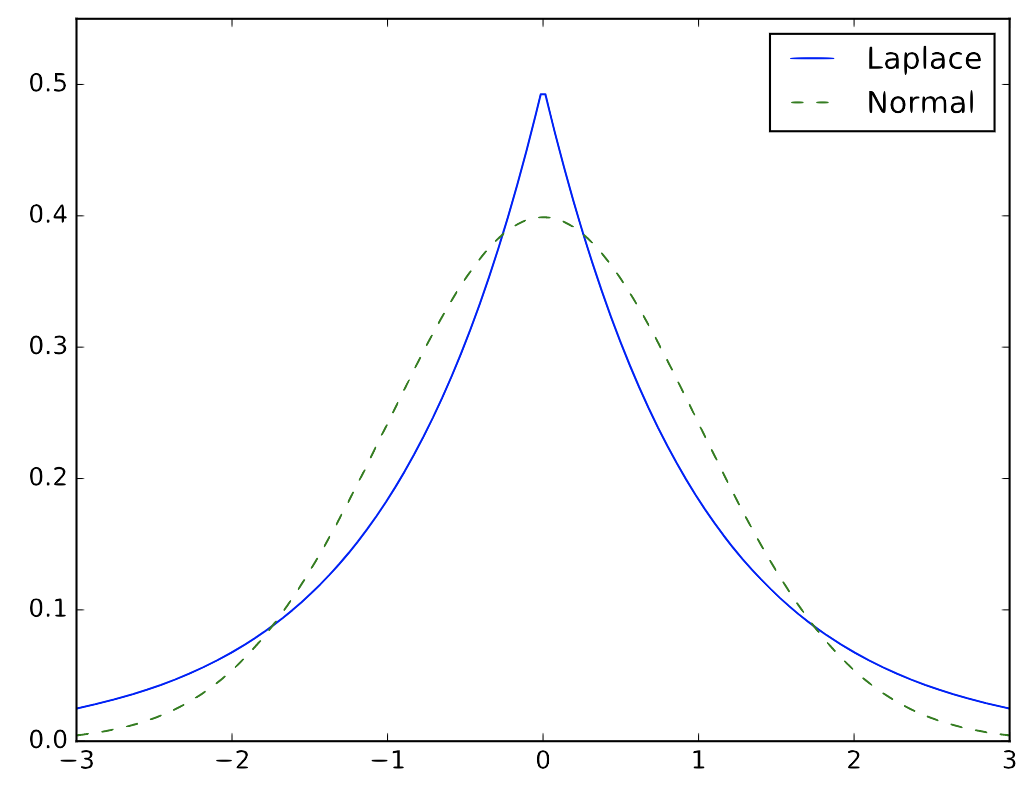
\includegraphics[width=.9\textwidth]{laplacen.png}
			\end{column}
			\begin{column}{.5\textwidth}
				$Pr(\eta = z) \sim$
			\end{column}
		\end{columns}
	
	Laplace noise has ``heavier tails'', meaning that it results in more outliers.
	
		This is a completely different justification for $\ell_1$ loss. 
\end{frame}

\begin{frame}
	\frametitle{bayesian regularization}
	\begin{center}
	\sout{assume all $\bs{\beta}$'s equally likely}	
	
	\textbf{Bayesian view:} Assume values in $\bs{\beta} = [\beta_1, \ldots, \beta_d]$ come from some distribution. 
	\end{center}

\begin{itemize}
	\item \textbf{Common model:} $\beta_i \sim N(0,\gamma^2)$, i.e. normally distributed, independent.
	\item Encodes a belief that we are unlikely to see models with very large coefficients. 
\end{itemize}
\end{frame}

\begin{frame}
	\frametitle{bayesian regularization}
	\textbf{Recall:}  want to choose $\bs{\beta}$ to maximize:
	\begin{align*}
		\Pr(\bs{\beta} \mid (\bv{X},\bv{y}) )  = \frac{\Pr((\bv{X},\bv{y}) \mid  \bs{\beta} ) \Pr(\bs{\beta} )  }{\Pr((\bv{X},\bv{y}) )} .
	\end{align*}
	\begin{itemize}
	\item We can still ignore the ``evidence'' term $\Pr((\bv{X},\bv{y}))$ since it is a constant that does not depend on $\bs{\beta}$.
	\item $\Pr(\bs{\beta}) = \Pr({\beta}_1)\cdot  \Pr({\beta}_2)\cdot \ldots \cdot \Pr({\beta}_d)$
	\item $\Pr(\bs{\beta})  \sim $
	\end{itemize}
\end{frame}

\begin{frame}
	\frametitle{bayesian regularization}
	Easier to work with the {\textbf{log likelihood}}:
	\begin{align*}
	&\argmax_{\bs{\beta}}\Pr((\bv{X},\bv{y}) \mid  \bs{\beta} ) \cdot \Pr(\bs{\beta} ) \\
	& = \argmax_{\bs{\beta}} \prod_{i=1}^n e^{-(y_i - \langle \bv{x}_i, \bs{\beta} \rangle)^2/\sigma^2} \cdot \prod_{i=1}^n e^{-(\beta_i)^2/\gamma^2} \\ 
	&= \argmax_{\bs{\beta}}  \sum_{i=1}^n -(y_i - \langle \bv{x}_i, \bs{\beta} \rangle)^2/\sigma^2 + \sum_{i=1}^d -(\beta_i)^2/\gamma^2\\
	&= \argmin_{\bs{\beta}}  \sum_{i=1}^n (y_i - \langle \bv{x}_i, \bs{\beta} \rangle)^2+ \frac{\sigma^2 }{\gamma^2}\sum_{i=1}^d (\beta_i)^2/\sigma^2.
	\end{align*}
	
	Choose $\bs{\beta}$ to minimize $\|\bv{y} - \bv{X}\bs{\beta}\|_2^2 + \frac{\sigma^2 }{\gamma^2}\|\bs{\beta}\|_2^2$!
	
	
	This is a completely different justification for ridge regularization. 
\end{frame}

\begin{frame}
	\frametitle{bayesian regularization}
	\textbf{Test your intuition:} What modeling assumption justifies LASSO regularization: $\min \|\bv{y} - \bv{X}\bs{\beta}\|_2^2 + \lambda\|\bs{\beta}\|_1$.
\end{frame}



\end{document} 








